\documentclass[11pt]{article}

\usepackage[english]{babel}
\usepackage{indentfirst}
\usepackage{graphicx}
\usepackage{subfig}
\usepackage[section]{placeins}

\usepackage{xcolor}
\usepackage{listings}
\usepackage{float}
\usepackage{capt-of}

\usepackage{hyperref}

\begin{document}

\begin{titlepage}
	\begin{center}
		\vspace*{1cm}
		
		\Large
		\textbf{Puzzle 2D - Wrong Products}
		
		\vspace{0.5cm}
		\large
		Segundo Projeto
		
		\vspace{1.5cm}
		
		\textbf{Hugo Miguel Monteiro Guimarães}\\
		\textbf{Beatriz Costa Silva Mendes}
		
		\vspace{5cm}
		
		Trabalho realizado no âmbito da\\
		Unidade Curricular de Programação Lógica
		
		\vspace{0.8cm}
	
		
\includegraphics[width=0.4 \textwidth]{feup_logo.png}
		
		\vspace{1.5cm}		
		
		\large
		Mestrado Integrado em Engenharia Informática e Computação\\
		Faculdade de Engenharia da Universidade do Porto\\
		Porto\\
		28	 de dezembro de 2020
	
	\end{center}
\end{titlepage}


\pagebreak
\tableofcontents

\pagebreak


\section*{Resumo} 
Este trabalho foi desenvolvido no âmbito da Unidade Curricular de Programação em Lógica, através do sistema SICStus Prolog, e o seu objetivo foi resolver um problema de decisão utilizando Programação de lógica com restrição sobre domínios finitos. O problema escolhido foi \textbf{\emph{Wrong Products}} e tem como objetivo colocar números numa grelha de modo a que cada linha e coluna contenha apenas 2 dígitos e que o produto entre os mesmos corresponda a um determinado valor no exterior da grelha, com variação de uma unidade.

\bigskip
\bigskip

\section{Introdução}

O Problema de Otimização escolhido ,\emph{Wrong Products}, tem como objetivo colocar números numa grelha de modo a que cada linha e coluna contenha apenas 2 dígitos e que o produto entre os mesmos corresponda a um determinado valor no exterior da grelha, com variação de uma unidade.

Este problema tem como objetivo a implementação de uma grelha matricial com restrições sobre linhas, colunas e toda a malha utilizando programação de lógica com restrições sobre domínios finitos.

\bigskip

Este artigo possui a seguinte estrutura:

\begin{description}

\item[Descrição do Problema:] Descrição com detalhe do problema de
otimização ou decisão em análise, incluindo todas as restrições envolvidas.

\item[Abordagem:] Descrição da modelação do problema como um Problema de Satisfação de Restrições(PSR)

\begin{description}

\item[Variáveis de Decisão] Descrição das variáveis de decisão e
respetivos domínios, assim como o seu significado no contexto do problema em análise.

\item[Restrições] Descrição das restrições rígidas e flexíveis do problema e a
sua implementação utilizando o SICStus Prolog.

\item[Visualização da Solução:] Explicação dos predicados que permitem
visualizar a solução em modo de texto.

\end{description}


\item[Experiências e Resultados] Análise de problema e resultados obtidos

\begin{description}

\item[Análise Dimensional] Exemplificação da execução de instâncias do problema com
diferentes dimensões e análise dos resultados obtidos.

\item[Estratégias de Pesquisa] Descrição de diferentes estratégias de pesquisa, comparando os resultados.

\end{description}


\item[Conclusões e Trabalho Futuro:] Conclusões obtidas pela realização do trabalho

\item[Referências] Referências bibliográficas utilizadas

\item[Anexo] Anexos de resultados úteis para a resolução do problema.

\end{description}

\bigskip
\bigskip

\section{Descrição do Problema}

Wrong Products é um problema de decisão. Este problema pretende descobrir se é possível colocar números numa grelha de modo a que cada que cada número apareça uma única vez, e que cada linha e coluna contenha unicamente dois números, e que o seu produto corresponda a uma unidade acima ou abaixo de um determinado valor no exterior da grelha associado à respetiva linha ou coluna.

\pagebreak

\section{Abordagem}

Wrong Products é um Problema de Satisfação de Restrições(PSR) e é modelado por:

\subsection{Variáveis de Decisão}

Na resolução deste problema, é necessário criar as seguintes variáveis:

\begin{description}

\item[Length - ] Tamanho da grelha, indicando o número de linhas e colunas. Estes valores são iguais dado que a grelha corresponde a uma matriz quadrada. O valor de \emph{length} é passado como argumento do predicado, pelo que o seu domínio varia conforme o pretendido pelo utilizador.

\item[RowValues - ] Lista com os valores iniciais cuja diferença entre o produto dos 2 valores da respetiva linha seja 1.

\item[ColValues - ] Lista com os valores iniciais cuja diferença entre o produto dos 2 valores da respetiva coluna seja 1.

\item[FinalRowValues - ] Lista com os valores finais cuja diferença entre o produto dos 2 valores da respetiva linha seja 1.

\item[FinalColValues - ] Lista com os valores finais cuja diferença entre o produto dos 2 valores da respetiva coluna seja 1.

\emph{RowValues}, \emph{ColValues}, \emph{FinalRowValues} e \emph{FinalColValues} possuem o mesmo domínio, todos os valores inteiros positivos que não sejam superiores ao produto entre os 2 maiores valores permitidos, que corresponde a:

\[(Length *2)*(Length * 2 - 1)\]


\item[ListOfLists - ] Lista de Listas contendo a grelha do problema. Pode ser interpretada como uma representação matricial do problema. Contém valores inteiros a serem multiplicados em cada linha e coluna, e zeros que correspondem a casas vazias.

\item[Transpose - ] Lista de Listas contendo a matriz transposta da grelha do problema. Tem como propósito facilitar a aplicação de restrições às colunas da grelha do problema.

\item[Table - ] Forma achatada de ListOfLists. tem como objetivo permitir a aplicação de restrições sobre toda a grelha. 

Dado que apenas podem existir 2 números por linha e coluna, o domínio de ListOfLists, Transpose e Table é o mesmo e corresponde a todos os valores inteiros entre 0 e \(2*Length\).



\end{description}

\subsection{Restrições}

\textbf{ all\_distinct\_except\_0(List)} Permite aplicar uma restrição a todos os valores da grelha, de modo a que, tal como o nome indica, todos os valores sejam distintos exceto os zeros. Desta forma é possível garantir que não há valores semelhantes e, simultaneamente, utilizar o valor zero como representação de uma casa não ocupada.

\bigskip

\textbf{line\_restriction(List,Amount)} Recebe como argumentos uma lista de listas e um valor inteiro \emph{amount}, e restringe a quantidade de zeros em cada linha de uma Lista de Listas, consequentemente garantindo que existem apenas 2 valores em cada linha. Este predicado é evocado duas vezes, a primeira para \emph{ListOfList}, e a segunda para \emph{Transpose}, de modo a que a restrição seja aplicada quer a linhas quer a colunas.

\bigskip

\textbf{multiplication\_restriction(ListOfLists,List)} Recebe uma Lista de Listas e verifica se o produto dos valores diferentes de zero de cada linha difere uma unidade em relação ao respetivo valor de uma Lista. Este predicado é evocado duas vezes, a primeira para \emph{ListOfList} e \emph{RowValues}, e a segunda para \emph{Transpose} e \emph{Colvalues}, garantindo que tanto o produto de uma linha como o de uma coluna cumprem a restrição da multiplicação enunciada anteriormente.

\pagebreak

\section{Visualização da Solução}

Ao selecionar a opção de execução do nosso programa (se quiser ver um dos problemas 
\textit{default} ou resolver um problema gerado aleatoriamente), primeiro é 
mostrado um problema por resolver, ou seja, com os espaços dentro da matriz em branco.
Este problema por resolver é obtido através do predicado \textbf{display}, que além
de demonstrar a solução, faz também um \textit{refresh} ao ecrã.
Posteriormente, quando o utilizador pede a solução do problema, esta é apresentada graças
ao predicado \textbf{displayWithoutClean}, que faz o mesmo que o predicado \textbf{display},
no entanto não faz um \textit{refresh} ao ecrã.

Ambos os predicados mencionados anteriormente imprimem os valores das colunas inicialmente
e imprimem recursivamente os valores da tabela juntamente com os valores por cada linha.

\section{Experiências e Resultados}

\subsection{Análise Dimensional} Incluir exemplos de execução em instâncias do problema com
diferentes dimensões e analisar os resultados obtidos.

Embora Wrong Products seja um problema apresentado sobre a forma de uma matriz quadrada de dimensão 4, resolvemos este problema de decisão dinamicamente, sendo possível fazer variar a dimensão da grelha e obter as soluções existentes, se possível.

O predicado \emph{generatePuzzle(Length,RowValues,ColValues)} recebe como argumento o parâmetro \emph{Length}, que corresponde à dimensão da matriz, gerando parâmetros aleatórios de \emph{RowValues} e \emph{ColValues} que garantem a existência de uma solução válida para o problema, sendo então possível gerar um problema resolúvel de qualquer dimensão.

O predicado \emph{solver(Length,RowValues,ColValues)} recebe como argumento as variáveis de decisão obtidas pelo predicado \emph{generatePuzzle}, obtendo uma solução possível para o problema. No fim, é chamado o predicado \emph{displayWithoutClean} que permite visualizar a solução do problema conforme explicado na secção anterior. Tal como o \emph{generatePuzzle}, possui como argumento a variável \emph{Length}, que indica a dimensão da matriz.


Exemplos de execução de um problema com diferentes dimensões encontram-se na secção de anexos



\subsection{Estratégias de Pesquisa}

Após encontrarmos uma forma de resolver o problema, decidimos analisar diferentes estratégias de pesquisa, de modo a obter uma solução da maneira mais eficiente.

Para tal ser possível, utilizamos os predicados \emph{reset\_time} e \emph{print\_time(Msg)} disponibilizados no \emph{Moodle} para obter tempos de execução do \emph{solver} do problema.

Deste modo, decidimos variar as opções de escolha de variável e valor do \emph{labeling} do \emph{solver} do nosso problema, analisando o tempo de execução da resolução de problemas de diferentes dimensões.
Concluímos então que a opção que gerava os tempos de execução da forma mais eficiente eram os valores default de \emph{labeling}:  \[labeling([leftmost, step, down, satisfy],Table)\]

As restantes combinações de valores testadas acabam por ser sempre menos eficientes que a \emph{default}, sendo a discrepância notável quando maior a dimensão do problema gerado.

O valor de \(labeling([max, step, down, satisfy],Table)\) surpreendeu-nos pela negativa, dado que não era possível resolver o problema com a dimensão 30, enquanto as outras combinações conseguiam calcular o resultado em frações de tempo inferiores a 1 segundo, o que o que nos permitiu entender a importância da busca por uma estratégia de pesquisa eficiente.

De seguida encontram-se 2 gráficos comparando tempos de execução de diferentes opções de pesquisa, fazendo variar a dimensão do problema.

\bigskip

\begin{center}

	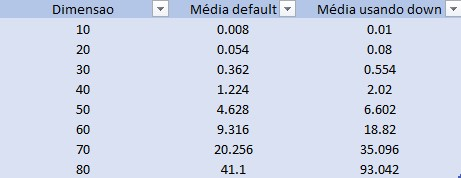
\includegraphics[width=0.8\textwidth]{tabela-comparacao.jpg}
	\captionof{figure}{Tabela com Média de Tempos de Execução, em segundos}

	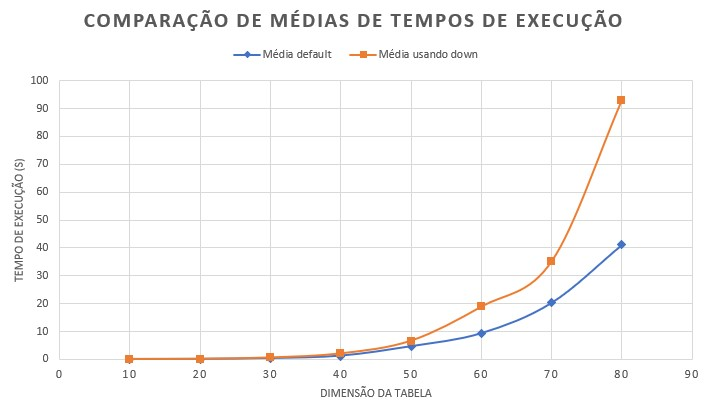
\includegraphics[width=0.8\textwidth]{grafico-comparacao.jpg}
	\captionof{figure}{Grafico com Média de Tempos de Execução}

\end{center}

\bigskip
\bigskip

\section{Conclusões e Trabalho Futuro} 
\paragraph{}
Este trabalho permitiu-nos	, por um lado, melhorar os nossos conhecimentos de Programação de lógica com restrições sobre domínios finitos, nomeadamente a sua utilização para resolução de Problema de Satisfação de Restrições. Por outro lado, também nos permitiu verificar na prática a influência de diferentes estratégias de pesquisa na resolução de um problema.

\paragraph{}
Os resultados obtidos demonstram que o problema proposto é facilmente resolúvel computacionalmente em tempos reduzidos, inferiores à décima do segundo para tabuleiros de dimensão inferior a 10, pelo que podemos concluir que tivemos sucesso no desenvolvimento da estratégia da solução do problema escolhido. Como seria de esperar, a complexidade temporal da solução proposta aumenta exponencialmente em função da dimensão do tabuleiro, pelo que o nosso programa tem dificuldade em encontrar soluções em tempo útil para malhas de dimensão superior a 60.

\pagebreak

\section{Referências} 


\href{https://logicmastersindia.com/lmitests/dl.asp?attachmentid=790&view=1}{We Are Puzzlers Club: Part 2 Instructions Booklet. (2019, August)}.

\bigskip

\href{https://moodle.up.pt/pluginfile.php/60682/mod_resource/content/13/PLR.pdf}{Programação em Lógica com Restrições. (2020, November)}. 

\bigskip

\href{https://moodle.up.pt/pluginfile.php/60683/mod_resource/content/10/PLR%20SICStus.pdf}{Programação em Lógica com Restrições
no SICStus Prolog. (2020, November)}. 
\pagebreak

\section{Anexos}

\begin{center}
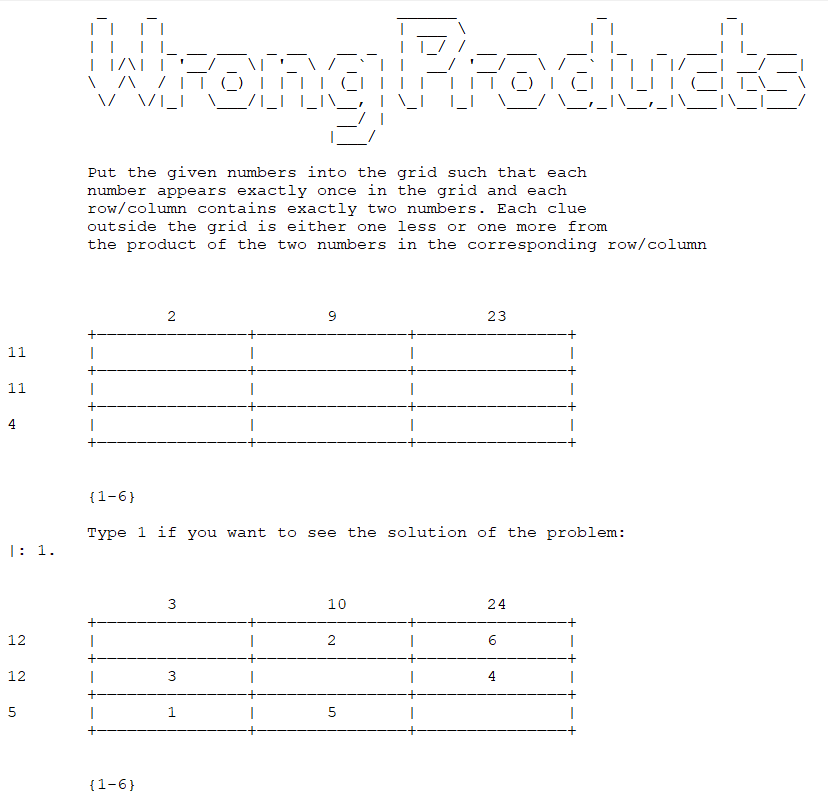
\includegraphics[width=0.65\textwidth]{dimension3.png}
\captionof{figure}{Execução do programa com dimensão 3}

\bigskip
\bigskip

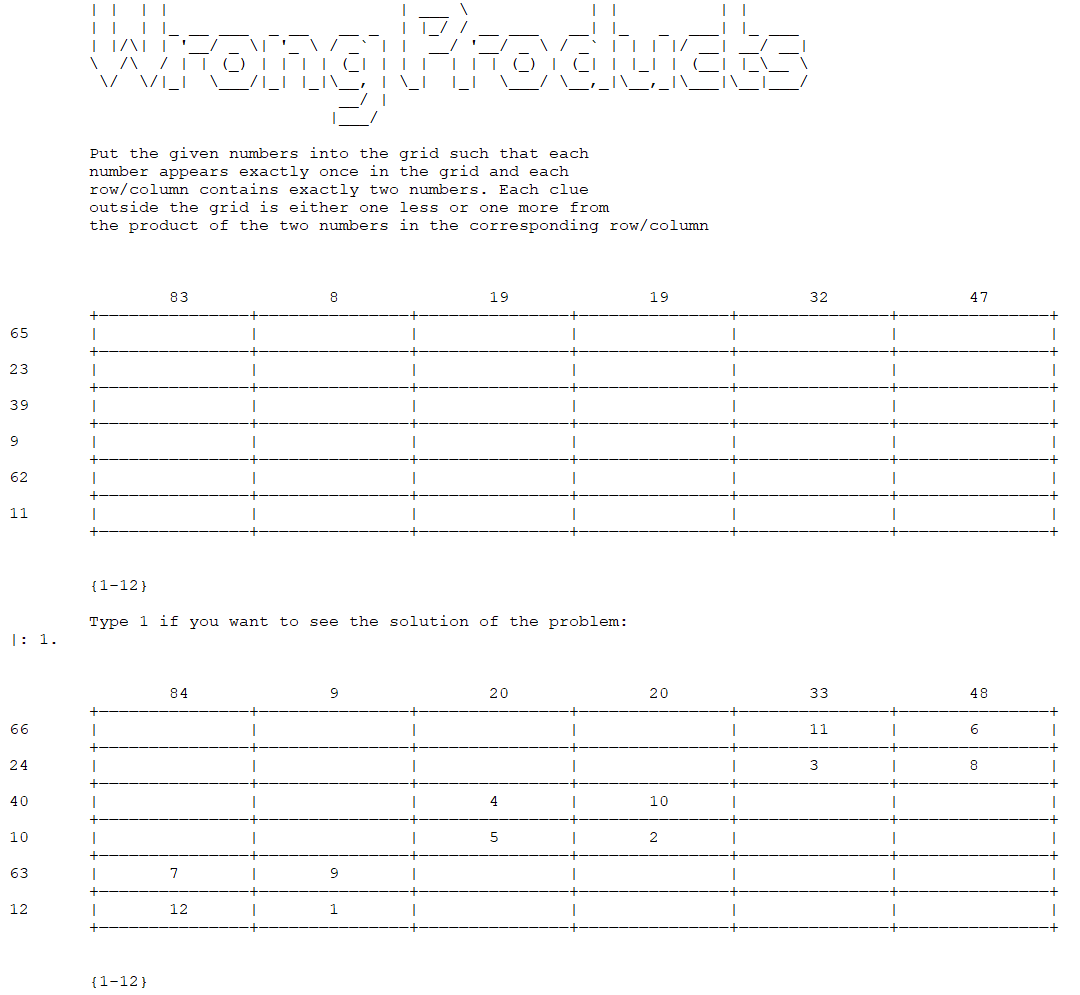
\includegraphics[width=0.65\textwidth]{dimension6.png}
\captionof{figure}{Execução do programa com dimensão 6}
\end{center}


\end{document}